\section{Case Studies}

We tested our technique on two representative problems. The full version of the Gap problem,
for which the running example in this paper is a simplified version, where the cost of replacing
the character $x_i$ with the character $y_j$ is given by $c_{ij}$ (\Cref{evaluation:gap spec});
and the Parenthesis Assignment problem, where the goal is a program computing
an optimal placements of parenthesis in a long chain of products, e.g. of matrices, where the input is
a cost function for performing each individual multiplication: initial cost $x_i$ for the $i$-th
element, $w_{ikj}$ is the cost for multiplying elements $[i,k)$ by elements $[k,j)$
 (\Cref{evaluation:paren spec}).

\begin{figure}
\[
  \renewcommand\arraystretch{1.5}
  \begin{array}{@{}l@{}l@{}l@{}}
    \lspan3{w :: ((J\times J)\cap{<})\to\R} \\
    \lspan3{w' :: ((K\times K)\cap{<})\to\R} \\
    G ~=~ \fix \theta\,i\,j\mapsto{}
      & \lspan2{0\big|_{i=0\land j=0} ~\Big/~ w'_{0j}\big|_{i=0} ~\Big/~ w_{i0}\big|_{j=0} ~\Big/~} \\
      & \min~\langle~ & \theta_{(i-1)\,(j-1)} + c_{ij},\\
      & & \min p\mapsto\theta_{pj}+w_{pi}, \\
      & & \min q\mapsto\theta_{iq}+w'_{qj} ~\rangle
  \end{array}
\]
\caption{\label{evaluation:gap spec}
  Specifications for the full version of the Gap DP problem.}
\end{figure}

\begin{figure}
\[
  \renewcommand\arraystretch{1.5}
  \begin{array}{@{}l@{}l@{}l@{}}
    \lspan3{x :: J\to\R} \\
    \lspan3{w :: (J\times J\times J)\to\R} \\
    E ~=~ \fix \theta\,i\,j\mapsto{}
      & \lspan2{x_{ij}\big|_{i+1=j} ~\Big/~} \\
      & \min k\mapsto\theta_{ik}+\theta_{kj}+w_{ikj} \\
  \end{array}
\]
\caption{\label{evaluation:paren spec}
  Specifications for the Parenthesis Assignment DP problem.}
\end{figure}


\subsection{old stuff}


At this point it can be noticed that step 1 is equivalent to the original
algorithm when given as input the prefixes of $x$ and $y$ whose length correspond to the
height and width of \qbox1.

With the other three steps, however, things are not so simple:
each of them is required to process some data in addition to the input.
For example, step 2 is required to read values from \qbox1, due to the expression
$G_{iq}$ (where $\scriptstyle 0\leq q<j$).
In order to reason more formally, we define $J$ and $K$ the index sets of the rows
and columns, respectively; $J_0$, $J_1$ for the top and bottom row indexes, respectively;
and $K_0$, $K_1$ for the left and right column indexes (\Cref{intro:slice G}).
The specifications for step 2 then take the following form:

\begin{equation}\LeftEqNo
\renewcommand\arraystretch{1.5}
\begin{array}{l@{}l}
	G_{\,(i : J_0)\,(j : K_1)} ~=~  \\
	\qquad
	\begin{cases}
		0                        & i=j=0 \\
		w'_{0j0}                 & i=0, j>0 \\
		w_{0i0}                  & i>0, j=0 \\
		\begin{array}{@{}l@{~}l}
		  \min\langle & \underset{0\leq (q:K) <j}\min ~ G_{iq} + w'_{qji}, \\
		              & \underset{0\leq (p:J_0) <i}\min ~ G_{pj} + w_{pij}~\rangle
		\end{array}              & i,j>0
	\end{cases}
\end{array}
\end{equation}

\medskip
Type annotations have been placed on $i$, $j$, $p$, and $q$ to define the regions
over which they range. $i:J_0, j:K_1$ means that the element $G_{ij}$
is always in \qbox2. Similarly, $G_{pj}$ is also in \qbox2. $G_{iq}$ is either in
\qbox1 or in \qbox2.


To address the situation, the algorithm designer would like to separate the parts
of the computation that read from \qbox1 from the parts that read from \qbox2.
This can be achieved here by splitting the $\min_{0\leq(q:K)<j}$ into two
ranges, according to the region in which $G_{iq}$ resides.

\begin{equation}\LeftEqNo
\renewcommand\arraystretch{1.5}
\begin{array}{l@{}l}
	G_{\,(i : J_0)\,(j : K_1)} ~=~  \\
	\qquad
	\begin{cases}
		0                        & i=j=0 \\
		w'_{0j0}                 & i=0, j>0 \\
		w_{0i0}                  & i>0, j=0 \\
		\begin{array}{@{}l@{~}l}
		  \min\langle & \underset{(q:K_0)}\min ~ G_{iq} + w'_{qji}, \\
		              & \underset{(q:K_1) <j}\min ~ G_{iq} + w'_{qji}, \\
		              & \underset{0\leq (p:J_0) <i}\min ~ G_{pj} + w_{pij}~\rangle
		\end{array}              & i,j>0
	\end{cases}
\end{array}
\end{equation}

\medskip
The path becomes clear: compute $\min_{(q:K_0)} ~ G_{iq} + w_{qj}$ first, for all $i$, $j$
in \qbox2. Then use the results to compute $G_{ij}$.

\begin{equation}\LeftEqNo
\renewcommand\arraystretch{1.5}
\begin{array}{l@{}l}
	G_{\,(i : J_0)\,(j : K_1)} ~=~  \\
	\qquad
	\textrm{let}~\psi_{ij} = \underset{(q::K_0)}\min ~ G_{iq} + w'_{qji} \\
	\qquad\textrm{in} \\
	\qquad
	\begin{cases}
		0                        & i=j=0 \\
		w'_{0j0}                 & i=0, j>0 \\
		w_{0i0}                  & i>0, j=0 \\
		\begin{array}{@{}l@{~}l}
		  \min\langle & \psi_{ij}, \\
		              & \underset{(q:K_1) <j}\min ~ G_{iq} + w'_{qji}, \\
		              & \underset{0\leq (p:J_0) <i}\min ~ G_{pj} + w_{pij}~\rangle
		\end{array}              & i,j>0
	\end{cases}
\end{array}
\label{intro:let in 2}
\end{equation}

\medskip
The second part in \eqref{intro:let in 2} starts to look similar to \eqref{intro:arbiter spec}:
in particular, the types of $p$ and $q$ are the same as those of $i$ and $j$.
In fact, if we set $\psi_{ij}=\infty$, we get \eqref{intro:arbiter spec} as a special case,
only with $J_0$ and $K_1$ instead of $J$ and $K$.
It therefore makes sense to write a version that generalizes both.

\begin{equation}\LeftEqNo
\renewcommand\arraystretch{1.5}
\begin{array}{l}
	A^{^{JK}}_{\,\psi ij} ~=~  \\
	\qquad
	\begin{cases}
		0                        & i=j=0 \\
		w'_{0j0}                 & i=0, j>0 \\
		w_{0i0}                  & i>0, j=0 \\
		\begin{array}{@{}l@{~}l}
		  \min\langle & \psi_{ij}, \\
		              & \underset{(q:K)<j}\min ~ A^{^{JK}}_{\psi iq} + w'_{qji}, \\
		              & \underset{(p:J)<i}\min ~ A^{^{JK}}_{\psi pj} + w_{pij}~\rangle
		\end{array}              & i,j>0
	\end{cases}
\end{array}
\label{intro:arbiter phase A}
\end{equation}

\medskip
And we can now rewrite \eqref{intro:arbiter spec} and \eqref{intro:let in 2} as
%
\begin{equation}
	G_{ij} ~=~ A^{^{JK}}_{\,(\infty^{J\times K})\,(i:J)\,(j:K)}
\end{equation}
%
\begin{equation}
\renewcommand\arraystretch{1.3}
\begin{array}{l@{}l}
	G_{\,(i : J_0)\,(j : K_1)} ~=~ 
	& \textrm{let}~\psi_{ij} = \underset{(q:K_0)}\min ~ G_{iq} + w_{qj} \\
	& \textrm{in}~A^{^{J_0K_1}}_{\,\psi ij}
\end{array}	
\label{intro:let in 2 using A}
\end{equation}

\newcommand\otherwise{\textrm{\small otherwise}}

\medskip
It takes a bit more insight to notice that \eqref{intro:let in 2 using A} can be further
generalized into:
%
\begin{equation}\LeftEqNo
\renewcommand\arraystretch{1.5}
\begin{array}{l@{}l}
	A^{^{JK}}_{\,\psi\,(i : J_0)\,(j : K_1)} ~=~ \\
	\qquad
	\textrm{let}~\psi'_{ij} = \begin{cases}
	  \begin{array}{@{}l@{}l@{}}\min\langle & \psi_{ij}, \\ & \!\underset{(q:K_0)}\min ~ A^{^{J_0K_0}}_{\,\psi iq} + w'_{qji}\rangle\end{array} & \langle i,j\rangle\mbox{ in }\qbox2 \\
	  \psi_{ij} & \otherwise
	\end{cases} \\
	\qquad\textrm{in}~
	A^{^{J_0K_1}}_{\,\psi' ij}
\end{array}
\label{intro:let in A 2}
\end{equation}

That is the core of the divide and conquer method: representing the output as a combination
of solutions to sub-problems, yielding an algorithm that is essentially
a recursive routine, or a set of mutually recursive routines. 
Once all the pieces fit together, it is possible to cut the space into arbitrarily small pieces,
that fit nicely in each core's local cache. This greately increases performance, as demonstrated
by~\citneeded{perhaps include a table with exact figures}. 
\todo{Find a way to make this statement earlier}

\medskip
We can apply similar treatment to \qbox3 and \qbox4:
%
\begin{equation}\LeftEqNo
\renewcommand\arraystretch{1.5}
\begin{array}{l@{}l}
	A^{^{JK}}_{\,\psi\,(i : J_1)\,(j : K_0)} ~=~ \\
	\qquad
	\textrm{let}~\psi'_{ij} = \begin{cases} 
	  \begin{array}{@{}l@{}l@{}}\min\langle & \psi_{ij}, \\ & \!\underset{(p:J_0)}\min ~ A^{^{J_0K_0}}_{\,\psi pj} + w_{pij}\rangle \end{array} & \langle i,j\rangle\mbox{ in }\qbox3 \\
	  \psi_{ij} & \otherwise \\
	\end{cases} \\
	\qquad\textrm{in}~
	A^{^{J_1K_0}}_{\,\psi' ij}
\end{array}
\label{intro:let in A 3}
\end{equation}

\begin{equation}\LeftEqNo
\renewcommand\arraystretch{1.5}
\begin{array}{l@{}l}
	A^{^{JK}}_{\,\psi\,(i : J_1)\,(j : K_1)} ~=~ \\
	\qquad
	\textrm{let}~\psi'_{ij} = \begin{cases} 
	  \begin{array}{@{}l@{}l@{}}\min\langle & \psi_{ij}, \\
         & \!\underset{(q:K_0)}\min ~ A^{^{J_1K_0}}_{\,\psi iq} + w'_{qji}\rangle \\
         & \!\underset{(p:J_0)}\min ~ A^{^{J_0K_1}}_{\,\psi pj} + w_{pij}\rangle \end{array} & \langle i,j\rangle\mbox{ in }\qbox4 \\
	  \psi_{ij} & \otherwise \\
	\end{cases} \\
	\qquad\textrm{in}~
	A^{^{J_1K_0}}_{\,\psi' ij}
\end{array}
\label{intro:let in A 4}
\end{equation}

Evidently there are some common sub-expressions. Defining
\begin{equation}
\renewcommand\arraystretch{1.3}
\begin{array}{l@{}l@{}l}
	B^{^{JK_0K_1}}_{\,\psi\,(i : J)\,(j : K_1)} ~=~ &
	  \min\langle & \psi_{ij}, \\ 
	&  & \!\underset{(q:K_0)}\min ~ \psi_{iq} + w'_{qji}\rangle \\[.8em]
	C^{^{J_0J_1K}}_{\,\psi\,(i : J_1)\,(j : K)} ~=~ &
	  \min\langle & \psi_{ij}, \\ 
	&  & \!\underset{(p:J_0)}\min ~ \psi_{pj} + w_{pij}\rangle 
\end{array}
\label{intro:spec of B,C}
\end{equation}

We can write \eqref{intro:let in A 2}, \eqref{intro:let in A 3}, \eqref{intro:let in A 4} as ---

\newcommand\qqquad{\qquad\qquad}

\begin{equation}\LeftEqNo
\renewcommand\arraystretch{1.5}
\begin{array}{@{}l@{}l}
    \lspan2{
	A^{^{JK}}_{\,\psi\,(i : J_0)\,(j : K_1)} ~=~ } \\
	\qqquad
	\textrm{let}~ & \psi'_{ij} = \begin{cases}
	  A^{^{J_0K_0}}_{\psi ij} & \langle i,j\rangle\mbox{ in }\qbox1 \\
	  \psi_{ij} & \otherwise
	\end{cases} \\[1.2em]
	& \psi''_{ij} = \begin{cases}
	  B^{^{J_0K_0K_1}}_{\psi' ij} & \langle i,j\rangle\mbox{ in }\qbox2 \\
	  \psi'_{ij} & \otherwise
	\end{cases} \\
	\lspan2{
	\qqquad\textrm{in}~
	A^{^{J_0K_1}}_{\,\psi'' ij} }
\end{array}
\label{intro:let in A 2 using B}
\end{equation}

\begin{equation}\LeftEqNo
\renewcommand\arraystretch{1.5}
\begin{array}{@{}l@{}l}
    \lspan2{
	A^{^{JK}}_{\,\psi\,(i : J_1)\,(j : K_0)} ~=~ } \\
	\qqquad
	\textrm{let}~ & \psi'_{ij} = \begin{cases}
	  A^{^{J_0K_0}}_{\psi ij} & \langle i,j\rangle\mbox{ in }\qbox1 \\
	  \psi_{ij} & \otherwise
	\end{cases} \\[1.2em]
	& \psi''_{ij} = \begin{cases}
	  C^{^{J_0J_1K_0}}_{\psi ij} & \langle i,j\rangle\mbox{ in }\qbox3 \\
	  \psi_{ij} & \otherwise
	\end{cases} \\
	\lspan2{
	\qqquad\textrm{in}~
	A^{^{J_1K_0}}_{\,\psi' ij} }
\end{array}
\label{intro:let in A 3 using C}
\end{equation}

\begin{equation}\LeftEqNo
\renewcommand\arraystretch{1.5}
\begin{array}{l@{}l}
	\lspan2{A^{^{JK}}_{\,\psi\,(i : J_1)\,(j : K_1)} ~=~} \\
	\qquad
	\textrm{let}~ & \psi'_{ij} = \begin{cases}
	  A^{^{J_0K_1}}_{\psi ij} & \langle i,j\rangle\mbox{ in }\qbox2 \\
	  A^{^{J_1K_0}}_{\psi ij} & \langle i,j\rangle\mbox{ in }\qbox3 \\
	  \psi_{ij} & \otherwise
	\end{cases} \\[1.8em]
	& \psi''_{ij} = \begin{cases}
	  B^{^{J_1K_0K_1}}_{\psi' ij} & \langle i,j\rangle\mbox{ in }\qbox4 \\
	  \psi'_{ij} & \otherwise
	\end{cases} \\[1.2em]
	& \psi'''_{ij} = \begin{cases}
	  C^{^{J_0J_1K_1}}_{\psi'' ij} & \langle i,j\rangle\mbox{ in }\qbox4 \\
	  \psi''_{ij} & \otherwise
	\end{cases} \\
	\lspan2{
	\qquad\textrm{in}~A^{^{J_1K_0}}_{\,\psi''' ij}
	}
\end{array}
\label{intro:let in A 4 using B,C}
\end{equation}

\begin{figure*}
\begin{center}
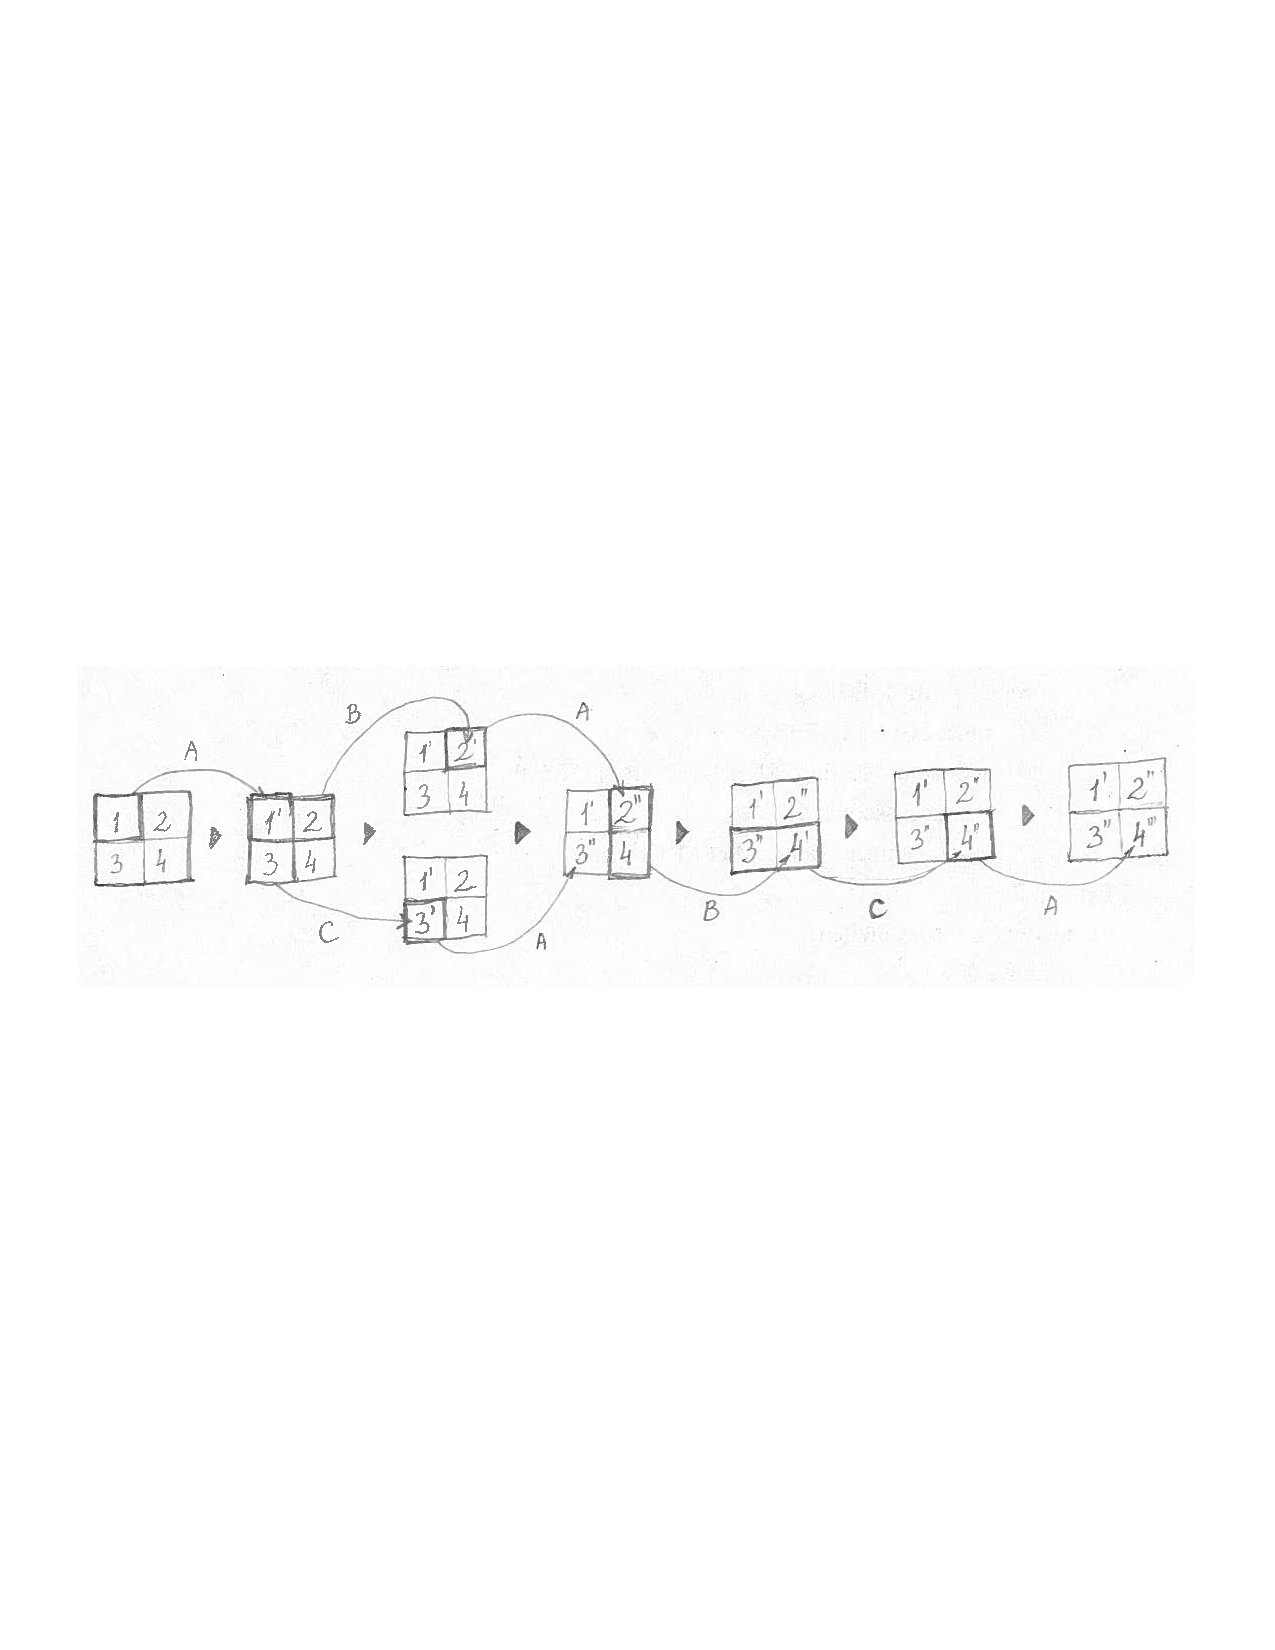
\includegraphics[width=.9\textwidth]{img/gap-stratify-A}
\end{center}
\caption{\label{intro:arbiter stratify A chain}}
\end{figure*}

This leads to the further stratified version shown in \Cref{intro:arbiter stratify A chain}.
The phases
$B$ and $C$ \eqref{intro:spec of B,C} are two more sub-problems that have to be addressed using the same slicing technique.
At first, it may seem that we have completed one task but created two; 
fortunately, $B$ and $C$ are much simpler instances\todo{for once, they are not recursive}
and are quite easy to develop.\todo{show this? Forget about this paragraph??}



\begin{center}$\vdots$
\end{center}


